\documentclass[times, utf8, diplomski, english]{fer}
\usepackage{booktabs}
\usepackage{amsmath}
\usepackage{nccmath}
\begin{document}


\thesisnumber{1417}
\title{Deep Learning Model for Base Calling of MinION Nanopore Reads}
\author{Marko Ratković}

\maketitle

% Ispis stranice s napomenom o umetanju izvornika rada. Uklonite naredbu \izvornik ako želite izbaciti tu stranicu.
\izvornik

% Dodavanje zahvale ili prazne stranice. Ako ne želite dodati zahvalu, naredbu ostavite radi prazne stranice.
\zahvala{Thanks ...}

\tableofcontents
\listoffigures
\listoftables

%%%%%%%%%%%%%%%%%%%%%%%%%%%%%%%%%%%%%%%%%%%%%%%%%%%%%%%%%%%%%%%%%%%%%%%%%%%%%%%%%%%%%%%
%% CHAPTER
\chapter{Introduction}

In recent years,  deep learning and usage of deep neural networks have significantly improved the state-of-the-art in many application domains such as computer vision, speech recognition, and natural language processing. 
In this thesis, we present application of deep learning in the fields of Biology and Bioinformatics for analysis of DNA sequencing data. 

DNA is a molecule that makes up the genetic material of a cell responsible for carrying the information an organism needs to survive, grow and reproduce. 
It is a long polymer of simple units called nucleotides attached together to form two long strands that spiral to create a structure called a double helix. The order of these bases is what determines DNA's instructions, or genetic code.

DNA sequencing is the process of determining this sequence of nucleotides. Originally sequencing was very expensive process but 
during the last couple of decades, the price of sequencing drastically dropped. A significant breakthrough occurred in May 2015 with the release of MinION sequencer by Oxford Nanopore making DNA sequencing inexpensive and available even for small research teams. 

Base calling is a process assigning sequence of nucleotides (bases) to the raw data generated by the sequencing device or sequencer. Simply put, it is a process of decoding the raw output from the sequencer.


\section{Objectives}
Goal of this thesis is to present novel approach for base calling of raw Nanopore sequencing data using deep learning convolutional neural networks.
\section{Organization}
\indent Chapter 2 gives more detailed explanation of the problem, background on nanopore sequencing and overview of state-of-the-art basecallers.

Chapter 3 describe used deep learning concepts in detail used later on in later chapters.

Chapter 4 goes into implementation details, training of the deep learning model and explains methods used to evaluate obtained results. 

Chapter 5 consists of the results of testing performed on different datasets as well as comparison with state-of-the-art basecallers.

In the end, the Chapter 6 gives a brief conclusion and possible future work and improvements of the developed basecaller.

%%%%%%%%%%%%%%%%%%%%%%%%%%%%%%%%%%%%%%%%%%%%%%%%%%%%%%%%%%%%%%%%%%%%%%%%%%%%%%%%%%%%%%%
%% CHAPTER
\chapter{Background}

\section{Sequencing}

Sequencing the entire genome of an organism is a difficult problem due to limitations of technology.
All sequencing technologies to date have constraints on the length of the strand they can process. 
These lengths are much smaller than the genome for a majority of organisms, therefore, whole genome shotgun sequencing approach is used. 
In this approach, multiple copies of the genome are broken up randomly into numerous small fragments that can be processed by the sequencer. Sequenced fragments are called reads.

Genome assembly is the process of reconstructing the original genome from reads and usually starts with finding overlaps between reads.
The quality of reconstruction heavily depends on the length and accuracy of the reads produced by the sequencer. Short reads make resolving repetitive regions practically impossible.

Figure \ref{fg:sequencing} depicts process of sequencing.

\begin{figure}[!ht]
	\begin{center}
		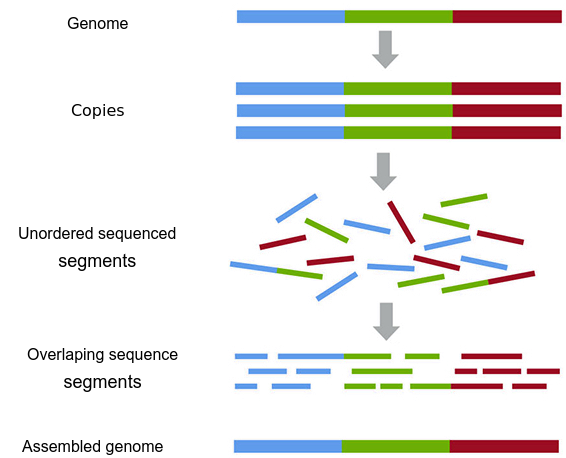
\includegraphics[width=0.6\textwidth]{./imgs/sequencing.png}
		\caption{Depiction of the sequencing process}
		\label{fg:sequencing}
	\end{center}
\end{figure}


Development of sequencing started with work of Frederick Sanger. In 1977, he developed the first sequencing method which allowed 
read lengths up to 1000 bases with very high accuracy (99.9%) at a cost of 1$ per 1000 bases[mile_skripta].
Second generation sequencing (IAN Torrent and Illumina devices) reduced the price of sequencing while maintaining high accuracy. Mayor disadvantage of these devices is read length of only a few hundred base pairs.
The need for technologies that would produce longer reads led to the development of so-called third generation sequencing technologies.
PacBio developed sequencing method that allowed read lengths up to several thousand bases but at a cost of accuracy. Error Rates of PacBio devices are ~10-15\%. 

Cost makes the main obstacle stopping widespread genome sequencing.
A significant breakthrough occurred in May 2015 with a release of MinION sequencer by Oxford Nanopore making sequencing drastically less expensive and even portable.


\section{Oxford Nanopore}

\subsection{Technology}

\subsection{Basecalling}

\begin{figure}[!ht]
	\begin{center}
		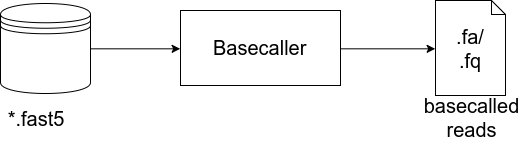
\includegraphics[width=0.5\textwidth]{./imgs/basecalling.png}
		\caption{Basecalling}
		\label{fg:basecalling}
	\end{center}
\end{figure}


\section{Existing basecallers}

Official basecaller for Nanopore reads is Metrichor. 

MetriKNOW - software that analyses signal as segments it into blocks called events. Events are described with lenght of the block, mean value of messured current and its variance.

Metrichor - uses events output from minknow and models HMM  - each state represents contex in the pore - 5 base pares. When transitioning from one state to an other - event is emited. By modeling emission probabilities and transition probabilities - from sequence of events, using viterbi algorithm is not difficult to determine most probable sequence expressed as series of transitions ih the model.
From states modeled as 5 bp it is impossible to model reppetitions of more than 5 bases.


Nancall - open source basecaller uses HMM approch like the original R7 Metrichor). Metrichor. Supports only R7 chemistry. 
Nanocall [7] was the first open-source basecaller for the MinION offered as an alternative to the proprietary Metrichor software. It was written in C++. Nanocall accepts the segmented signal from minKNOW and assigns
k-mers to the events using a hidden Markov model (HMM). A

DeepNano - first open source basecaller based on neural networks. It uses bidirectional rnn. Originaly supported R7 chemistry, later on support for R9.4 and R9.5 was added.

Deepnano is a python package built on the Theano framework, and uses a deep recurrent neural network (RNN) model to call bases. ONT has also moved towards RNN basecalling and this is now the main method for calling R9 reads

DeepNano Before Metrichor made its own switch from HMM- to RNNbasecalling,
the open-source basecaller DeepNano [8] already implemented a
form of RNN basecalling, booking a significant improvement in accuracy with
respect to the then-current Metrichor version (corresponding to the SQK-MAP-
006 kit, late 2015).
 DeepNano was written in Python, using the Theano library
[50]. The RNN employed in DeepNano consists of 3 hidden layers of 100 units per
layer for 1D basecalling and 4 hidden layers of 250 units for 2D. Rather than
LSTM-nodes, as currently used in Metrichor basecallers, DeepNano implements
gated recurrent units (GRUs) [51] to accou


NanoNet Nanonet provides recurrent neural network basecalling via CURRENNT.

Albacore -Albacore is a C++ project designed to provide a high-performance end-to-end analysis pipeline that can be run on (potentially) any platform. Albacore is currently only available through the ONT Developer Channel to users who have signed the Developer terms and conditions. 

Scrappie - A proprietary basecaller by Metrichor and platform for ongoing
development, Scrappie was the first basecaller reported to specifically address
homopolymer basecalling. It was just recently released on their official GitHub.



%%%%%%%%%%%%%%%%%%%%%%%%%%%%%%%%%%%%%%%%%%%%%%%%%%%%%%%%%%%%%%%%%%%%%%%%%%%%%%%%%%%%%%%
%% CHAPTER
\chapter{Methods}
Thesis Methods.
\section{Arhitecture}
Describe classic arhitecture: convolution, pooling, activation
Zasto svaki dio itd
Batch Normalization 
Iterativno se treniraju.
\subsection{CNN}

\begin{gather*}
y_i = w_1 * x_{i-1} + w_2 * x_{i} + w_3 * x_{i+1}
\end{gather*}
\begin{figure}[!ht]
	\begin{center}
		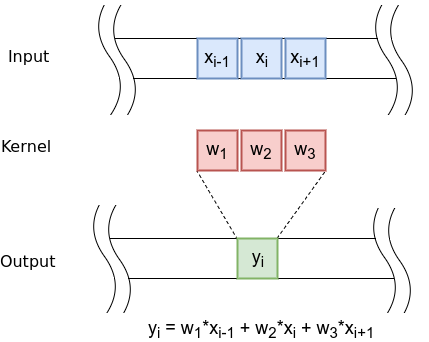
\includegraphics[width=0.5\textwidth]{./imgs/convolution.png}
		\caption{Convolution layer, kernel size 3}
		\label{fg:convolution}
	\end{center}
\end{figure}

\subsection{Residual Networks}
Vanishing gradient problem
\subsection{Gated Residual Networks}
Why not use only needed - distribution of gates

\section{CTC Loss}
\subsection{Definition}
\subsection{Decoding}


%%%%%%%%%%%%%%%%%%%%%%%%%%%%%%%%%%%%%%%%%%%%%%%%%%%%%%%%%%%%%%%%%%%%%%%%%%%%%%%%%%%%%%%
%% CHAPTER
\chapter{Implementation}
\section{Deep Learning model}
\section{Training}

To train described model we need to obtain dataset that consist of sample pairs $(X_i, Y_i)$ where $(X_i)$ is input signal and $Y_i$ is output sequence. 
One of the mayor issues is determining correct output for given signal. One option is to use existing basecaller like Metrichor to determine output sequences. 

 




Supervised learning so for need to specify dataset that for each input signal we need specify desired sequence of bases.
{Xi, Yi} where len of X and len of Yi are not specified.

For each input file, ground truth is not specified. If we use output of Metrihor or any other basecaller we limit our model to
obtain accuracy of used basecaller in best case. We limit our train data to only sequencing data of know organisms (organisms with know reference genome) and try to correct data by aligning the read produced by metrichor or any other basecaller to reference genome. Alignment destination is used as target sequencing in training. 
Using Metrichor basecalled data we can determine for each called event values such as start in signal, length of event, k-mer state in the pore and using move field change of k-mer from previous state. 

Used dataset for training consists of raw signal from fast5 files split raw data into blocks of size $l$.
For each block it is easy to determine basecalled events from Metrichor that belong to particular block using start information and from those events basecalled sequence. 


$block\_index =  \frac{event_{start} * sampling\_rate}{block\_size}$

Full basecalled sequence is aligned to the reference genome and alignment was obtained. For each block target sequence is determined from alignment information.

Figure X shows how for given signal block


Figure bla shows augmentation of data.

To eliminate possibility of overfitting to the know reference, model is trained and tested on reads that align to different regions of reference genome and those regions should not overlap. Also test is conducted on separate set of sequencing data for different organism than the one used for training. 

\begin{figure}[!ht]
	\begin{center}
		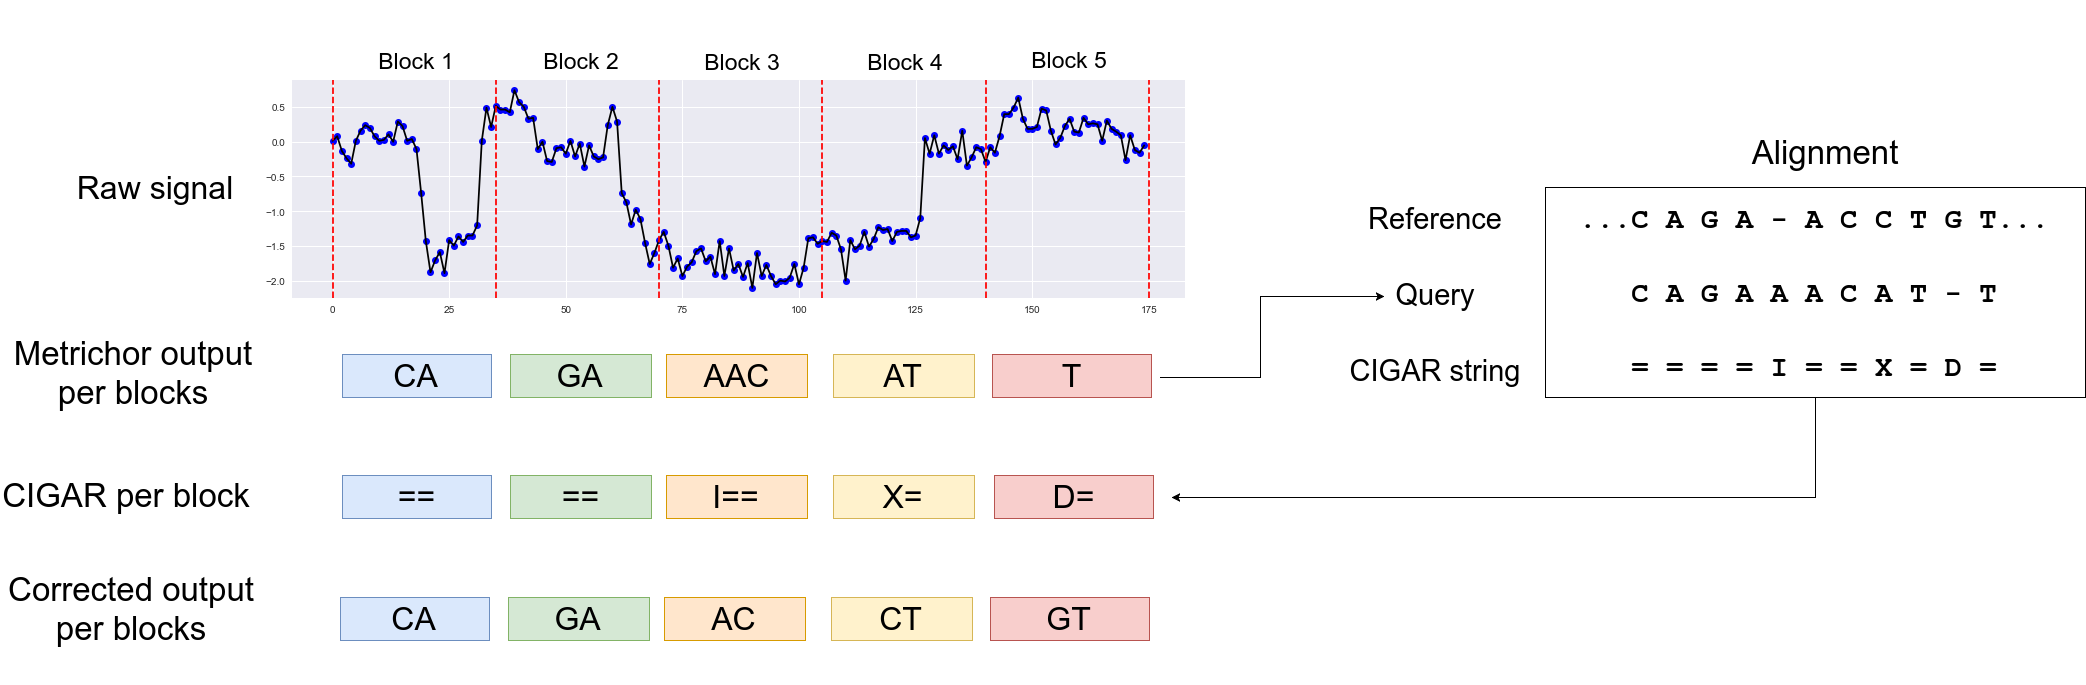
\includegraphics[width=1\textwidth]{./imgs/train_data_correction.png}
		\caption{Dataset preparation}
		\label{fg:data_correction}
	\end{center}
\end{figure}
\begin{figure}[!ht]
	\begin{center}
		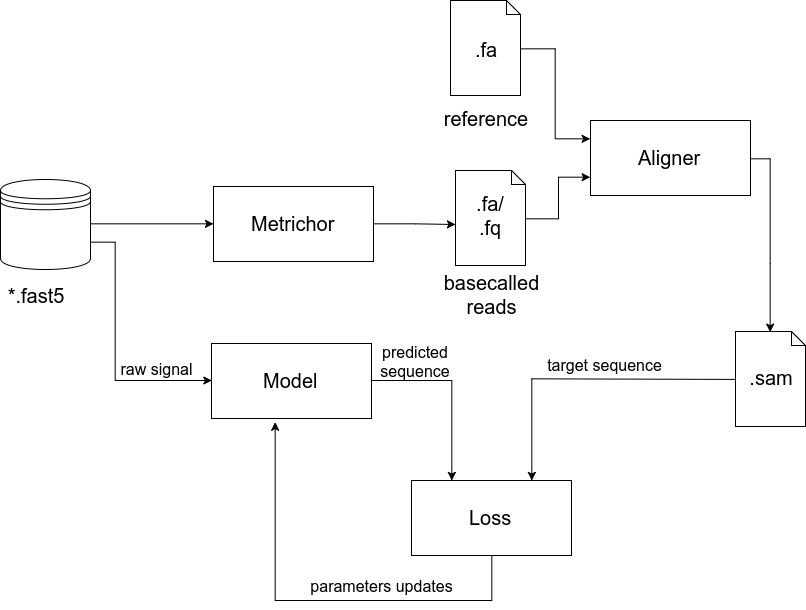
\includegraphics[width=0.7\textwidth]{./imgs/train_pipeline.png}
		\caption{Overview of training pipeline}
		\label{fg:train_pipe}
	\end{center}
\end{figure}
\section{Evaluation methods}
To evaluate trained model we base call test set, align those reads to reference and calculate various statistics on align data.
From cigar string it is easy to calculate following:

\begin{gather*}
read\_len =  n\_matches + n\_missmatches + n\_insertions \\
match\_rate = \dfrac{n\_matches}{read\_lenght} \\
missmatch\_rate = \dfrac{n\_missmatches}{read\_lenght}\\
insertion\_rate = \dfrac{n\_insertions}{read\_lenght}\\
deletion\_rate = \dfrac{n\_deletion}{read\_lenght}\\
match\_rate = \dfrac{n\_matches}{read\_lenght}\\
\end{gather*}

Results are calculated for each read in test dataset and mean value and standard deviation is expressed for the whole dataset.

To validate consistency of a basecaller, basecalled data is aligned to the reference genome and consensus sequence is called from all reads covering single position. Consensus sequence is compared with the reference genome and following measures are calculated:
\begin{gather*}
identity\_percentage =  100 * \dfrac{n\_correct\_bases}{reference\_lenght} \\
match\_rate = \dfrac{n\_correct\_bases}{consensus\_lenght} \\
snp\_rate = \dfrac{n\_snp}{consensus\_lenght}\\
insertion\_rate = \dfrac{n\_insertions}{consensus\_lenght}\\
deletion\_rate = \dfrac{n\_deletion}{consensus\_lenght}\\
\end{gather*}

\begin{figure}[!ht]
	\begin{center}
		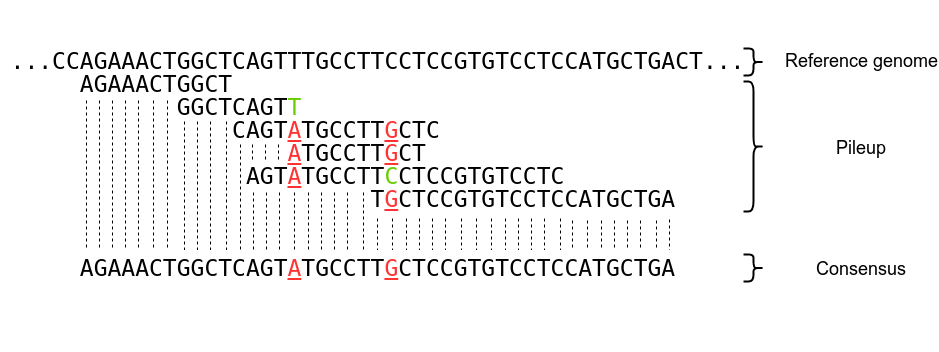
\includegraphics[width=0.8\textwidth]{./imgs/consnesus.png}
		\caption{Consensus from pileup}
		\label{fg:consensus}
	\end{center}
\end{figure}


\begin{figure}[!ht]
	\begin{center}
		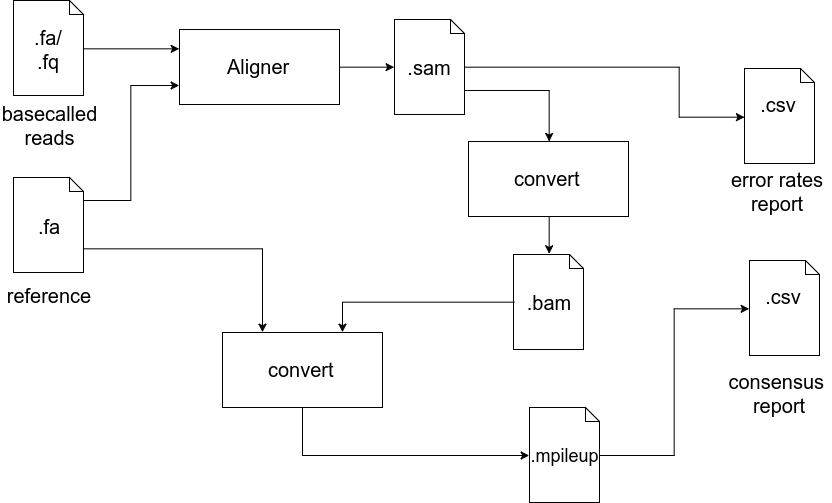
\includegraphics[width=0.7\textwidth]{./imgs/evaluation_pipeline.png}
		\caption{Overview of evaluation pipeline}
		\label{fg:eval_pipe}
	\end{center}
\end{figure}

\section{Technologies}

Overall solution was implemented in Python programing language. Described model is implemented using TensorFlow. Tensorflow is an open source software library for numerical computation using data flow graphs developed by Google.  TensorFlow, even tho is considered low-level framework offers implementations of higher level concepts (layers, losses, and optimizers) which makes it great for prototyping while keeping it modular and extensible for highly specific tasks as well.

Tensorflow offers efficient GPU implementations of various layers and losses but as of version 1.2 lacks GPU implementation of used CTC loss, so WARP-CTC (https://github.com/baidu-research/warp-ctc) was used. It offers both GPU and CPU implementations as well as bindings for Tensorflow.

For alignment tasks, developed tool offers support for GraphMap and BWA but can easily be extended with any other aligner that outputs results in Sam file format.

SAMTools(link) and its python bindings PySam(link) were used for conversions between various file formats used in Bioinformatics.

Docker was used for automating the deployments on different machines. It helps us resolve problem know as  "dependency hell"(link)  keeping all dependencies in single container thus eliminating possible conflict between packages on host OS.
Nvidia docker was used for GPU support.

All training was done on the server with  Intel(R) Xeon(R) E5-2640 CPU, 600 GB of RAM and NVIDIA TITAN X Black with 6GB of GDDR5 memory and 2880 CUDA cores.
%%%%%%%%%%%%%%%%%%%%%%%%%%%%%%%%%%%%%%%%%%%%%%%%%%%%%%%%%%%%%%%%%%%%%%%%%%%%%%%%%%%%%%%
%% CHAPTER
\chapter{Results}
\section{Data}
\section{Error rates per read}
\section{Consensus analysis}

%%%%%%%%%%%%%%%%%%%%%%%%%%%%%%%%%%%%%%%%%%%%%%%%%%%%%%%%%%%%%%%%%%%%%%%%%%%%%%%%%%%%%%%
%% CHAPTER
\chapter{Conclusion}
Conclusion.



%%%%%%%%%%%%%%%%%%%%%%%%%%%%%%%%%%%%%%%%%%%%%%%%%%%%%%%%%%%%%%%%%%%%%%%%%%%%%%%%%%%%%%%
%% DONE
\bibliography{references}
\bibliographystyle{plainnat}

\begin{abstract}
Abstract.

\keywords{Keywords.}
\end{abstract}

% TODO: Navedite naslov na hrvatskom jeziku.
\hrtitle{Model dubokog učenja za određivanje očitanih baza dobivenih uređajem za sekvenciranje MinION}
\begin{sazetak}
Sažetak na hrvatskom jeziku.

\kljucnerijeci{Ključne riječi, odvojene zarezima.}
\end{sazetak}

\end{document}
